% !TeX root = ../main.tex
% Add the above to each chapter to make compiling the PDF easier in some editors.

\chapter{Foundations}\label{chapter:foundations}
\section{Enterprise Architecture Management} 

This chapter provides a theoretical overview of the discipline Enterprise Architecture Management. The most important concepts, related fields and its challenges related to EA are described in this chapter.

The aim is to describe the EAD process of organizations. This section will present the specific EA information sources and the key problems regarding the EAD. First EAM is defined and the stakeholders are mentioned. Then the different use cases of EAM will be presented. Since documenting the current state of the enterprise IT landscape is one of the uses cases, the different approaches found in the literature for automating that documentation process are presented.

%1.	Motivation. Um was geht es? In welchem Bereich befinden wir uns?
%2.	Problemstellung. Welche Herausforderungen leitest du aus (1) ab?
%3.	Lösungsziel. Welches Problem in (2) möchtest du genau lösen? 
%4.	Lösungsansatz. Wie möchtest du das Problem in (2) lösen?
%5.	Forschungsfragen. Welche Herausforderungen musst DU lösen um das Lösungsziel zu erreichen.
%6.	Evaluationsumgebung. In welche Umgebung kannst du deinen Lösungsansatz evaluieren? Welche Tools stehen %dir zur Verfügung?
%7.	Nächste Schritte.

\subsection{EAM Definition}
The term Enterprise Architecture Management is composed of three words: Enterprise, Architecture and Management.
According to ANSI/IEEE Std 1471-2000 architecture is defined as ‘the fundamental organization of a system, embodied in its components, their relationships to each other and the environment, and the principles governing its design and evolution.’
%Enterprise Architecture definition
Applying the previous mentioned definition to the context of enterprises, the EA refers to the fundamental organization of an enterprise, embodied in its components (e.g. organizational units, stakeholders, locations, business processes), their relationships to each other, the principles, methods and models that are used in the design and realization of the enterprise’s organizational structure.
\hl{(Buckl 2009)}
Additionally, the term management according to Mary Parker Follet refers to ‘the art of getting things done through people’ \hl{(van Aken 2005)}.
\hl{(Buckl 2009)}
\hl{(Jonkers 2006)}
In summary the three terms results to the following definition: EAM is promoted as an instrument to improve alignment of business and IT, ideally suggesting a common language and a framework across the company to determine  which business and technical domains, business processes, information systems and technical building blocks are used conveying a holistic view of the entire organization to realize cost savings potentials, and increase availability and fault tolerance.
\hl{(Hauder 2012)}
\hl{(Hanschke 2006)}

\subsection{EAM Stakeholders}
For a successful operation of EAM all relevant stakeholder groups need to be identified and involved.
When analyzing which stakeholder groups play a role in the organizations EAM initiative central functions, departments and project organizations as well as IT and external organizations have to be included. 
%The following questions can help for determine the stakeholder-groups: Who is the contracting authority? What concerns are associated with EAM? Who is the data supplier?
Figure \hl{XXX} shows an overview of the stakeholder groups that typically influence, have an interest or can benefit from EAM. \hl{(Hanschke ???)}
\begin{figure}[htpb]
  \centering
  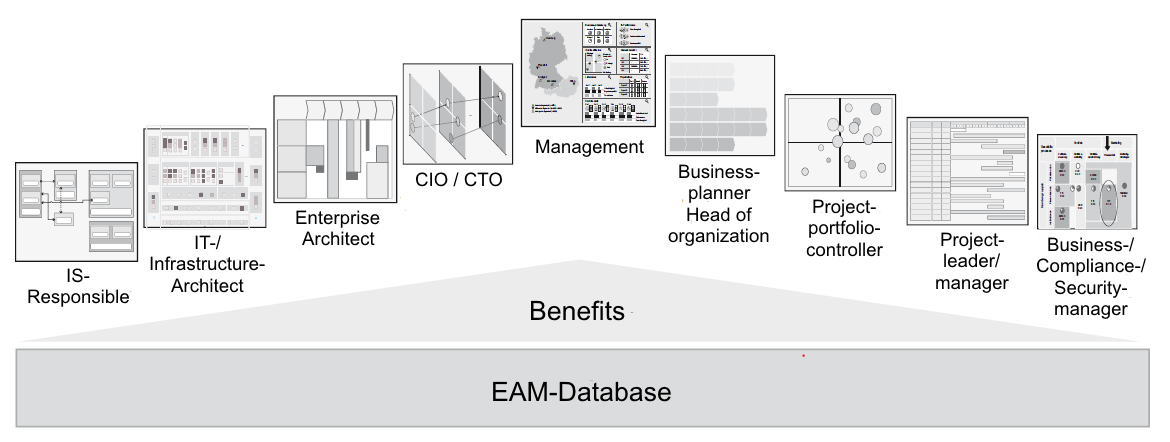
\includegraphics[width=0.8\textwidth]{figures/eam-stakeholder.png}
  \caption{ \hl{In Anlehnung an}Different stakeholder groups with interest in EAM~\parencite{Hanschke 2013}}
  \label{fig:Differet stakeholder groups with interenst in EAM}
\end{figure}

The following list shows stakeholder groups that are often involved in EAM initiatives in practice. The structuring is based on the TOGAF categories:\hl{(TOGAF Quelle)}
\begin{itemize}
    \item Corporate Functions
    \item End-User Organization
    \item Project Organization
    \item System Operations
    \item Externals
\end{itemize}

Not all categories are explained in detail. Only some stakeholder groups relevant for further sections of this work will be described briefly. These are named below and their tasks and EAM concerns are also explained. Some category mappings may vary by company. For example, enterprise architects are assigned to the stakeholder category IT.

\subsubsection{Corporate Functions}
\textbf{CIO (CTO)}: How are we performing on delivering our strategic goals? The CIO (CTO) covers the strategic corporate planning and definition of long-term target and framework requirements as well as planning and control systems and the corporate organization. The benefits of an EAM initiative is to ensure an optimization of the day-to-day business for the CIO (CTO) gathering a cross-company information report from the EAM database to provide the implementation of the corporate/enterprise goals.

\subsubsection{End-User Organization}
\textbf{Business manager}(including head of business units or areas and department heads): responsible for increasing the business IT alignment and further development of business and business architecture. Business managers endeavour to discover and remove technical redundancies and divisional differences in business processes and business capabilities and their IT support.

\subsubsection{Project Organization}
\textbf{Project leader or managers}: Responsible for the operative planning and control of a project. The expected benefits are reduced project preparation and input for project execution as well as input for operational planning and control of the project.
In addition to project managers, other stakeholder groups of a project organization may also benefit from EAM results. Examples include business analysts, software architects or solution architects. Solution architects often ensure the proper implementation of the development planning in projects through collaboration or review. 
%In collaboration with the project managers the channels of the offered %product is decided Which products will we offer via which channels? What %is the impact of making a change? What are the dependencies?

\subsubsection{System Operations}
\textbf{Enterprise Architects}: Main resposible for implementing and desgining and EAM initiative. Also in charge for the implementation of technical standards and principles and their use in the information system landscape and in the operational infrastructure as well as operational infrastructure development and the provision of SLAs at the operational infrastructure level.
%Which capabilities require investment to deliver our goals?


\subsubsection{Externals}
This category includes partners and suppliers, such as outsourcing service providers. The application of EAM to this category is the improvement of technical standards and specifications for the target development as input and framework conditions for services. The analysis of dependencies and effects of changes and the fulfillment of SLAs are also covered.

%Other stakeholder questions:
%Which applications are at risk from end-of-life technology?
%Which applications get replaces when?
%Which risks require mitigation? What are our greatest threats?

\subsection{EAM Use Cases}

% EA MetaModel
% use case areas
% Dependency management

In regard to the discipline EAM the use case types can be divided into two categories: operational and strategic use cases. This section will only list some key uses cases.

%Operational use cases
\subsubsection{Operational EAM use cases}
Operational use cases aim to support the current business cost-effectively and reliably with the help of IT, while continuously improving the IT support. The main challenges are: cost reduction, to reduce complexity of the IT landscape, the optimization of day-to-day business and identify risks. \hl{(Hanscke 2013)}.

As mentioned above only key uses cases are named in this section. Here is a list of some operational use cases:

%Metamodel hervorheben. Metamodel für abhängigkeiten
\textbf{Meta model as a common language}: Before gathering the EA data about the current state, an meta model of the architecture has to be defined, which describes the elements and relationships in between constituting the EA meta model to enable a common language across the organization. Collecting information from different layers requires the involvement of a multitude of stakeholders, e.g. business process owners, project managers, business architects, etc. Although working for the same organization, the definitions used by these stakeholders differ widely. This communication problem is often referred to as the communication gap between business and IT \hl{(Lankes 2008, Schekkerman 2004)}. This gap restricts adequate communication and collaboration in the EA management process.\hl{(Buckl et al. 2008)}. There are often more interactions between IT and business, as expected. To overcome this gap an EAM common language is needed. The resulting metamodel is used as the reference in the dialogue with the both parties.\hl{(Hanschke 2013)}

\textbf{EA Documentation}: In order to enable EAM and its life cycle, the current (as- is) state of the EA has to be documented. The different elements and layers covering business, organizational and infrastructure aspects have to be enclosed to provide a holistic view on the enterprise. The information gathered about the current situation, enables the planing for future states. Complementing the current and planned states of the EA an ideal target (to-be) state should be envisioned, which can be derived from the long-term vision of the enterprise. \hl{(Buckl et al. 2008)}. This use case will be described in detail in \subsectionautorefname{} Enterprise Architecture Documentation.

\textbf{Standardization and homogenization}: Definition of technical standards and monitoring of compliance and promotion of implementation. The goal of this use case is to reduce the IT complexity supporting the re-usability of proven technical building blocks. This increases the technical quality. The standardization and homogenization of technical standards concludes to a continuous cost reduction through the use of economies of scale and the bundling and reduction of the different know-how expertise.\hl{(Hanschke 2013)}

\textbf{Project portfolio management}: Creation of transparency about applications to optimize the support of business through IT and the planification of the roadmap for target architecture, ensuring the implementation of planned future development, IT consolidation and compliance in planning, prioritization, and overall governance and monitoring of the project portfolio. Through targeted management of project resources costs and also the IT complexity can be reduced.\hl{(Hanschke 2013)}

\textbf{Demand Management}: Planning and controlling the flow of strategic and operational business requirements for implementation through demand management. Demand Management translates the requirements between business and IT. As a bottleneck for the planning and control of the implementations of the business, it ensures that the technical goals and business requirements are adequately implemented.

%Strategic use cases
\subsubsection{Strategic EAM use cases}
Strategic use cases intent to improve systematically the development and strategic alignment of the different responsible. The main challenges are the setting of specifications and guarantee the compliance (EA Governance) and the progression of Business-Innovation and -Transformation.

\textbf{IS-Portfoliomanagement}: Identification of the potentials for the optimization in the IT landscape through the analysis of the architecture. One of the goals is to reduce the IT complexity through continuous IT consolidation and thus a sustainable reduction of IT costs. Another goal is to increase business IT alignment by evaluating the contribution of the IT to the business.

\textbf{Business-Transformation}: Standardization and homogenization of the future IT landscape
concerning the implementation of enterprise and IT strategy. The assurance of decisions can be ensured through the analysis of the dependencies and the effects of the IT landscape in relation to the business landscape.

According to the ANSI/IEEE Std 1471-2000 the main tasks of EAM are documentation (operational), communication (operational), and analysis of architectures (strategic). The following section will give a general outline of the enterprise architecture documentation.


\section{Enterprise Architecture Documentation} 

EAM begins with the documentation of the current state according to the defined EA metamodel to  derive future plans for an improved EA. Organizations endeavour with the documentation of the current state due to the complexity of enterprise architecture. This section will provide an overview of the enterprise architecture documentation process.

\subsection{Definition}

This first core product of EAM is the documentation of the current implementation of business processes, IT systems, and infrastructure (Schmidt and Buxmann 2010; Lankhorst et al. 2009; Kaisler et al. 2005; van der Raadt and van Vliet 2008). It needs to provide a current (PQ1a) and complete (PQ1b) view of the as-is architecture providing the right degree of detail (PQ1c) (Schmidt and Buxmann 2010; Foorthuis et al. 2010; Aier et al. 2011; Riege and Aier 2009; Winter and Fischer 2007; Aier and Schelp 2009; Bricknall et al. 2006; Schmidt and Buxmann 2010; Winter and Fischer 2007; Pulkkinen 2006). 

\subsection{Information Sources}
A survey conducted by \hl{Farwick} presents the major information sources for an EAD. This survey was done to provide an comprehensive analysis of possible information sources and their appropriateness for EA since research activities still seek to automate the data collection process.

The information sources correspond to the tools used by the participants of the survey. In addition, the participants also expressed their concerns regarding the EA relevant data delivered by the tool in respect of the following data properties in the EA context: actuality, completeness, correctness and granularity \hl{Farwick 2013}

\subsubsection{Network Scanners and Monitors}
%include source [4] of farwick 2013
The most common potential information source for an automated EAD are Network Scanners and Monitors. Operations teams often use these sources to monitor the infrastructure and its performance. As analyzed in the survey more than 60 percent of all organizations use Network Scanners.
Relevant data for network scanners are servers, applications and databases. However, the data gathered from this sources is too granular. The data can then not me mapped to the EA meta model. Nonetheless the correctness and the actuality of the data are considered positive. Since network scanners cannot cover all technologies the quality  of the collected data is worst of all information sources.

\subsubsection{Configuration Management Database}
Configuration Management Databases (CMDBs) are databases that store relevant information about hardware instances used in an organization's IT services and the relationships between those instances and the related incidents at an operational level.\hl{ITIL}
A CMDB should contain data about server, database and application instances. This data is mostly colleected and maintained manually. Same as with the network scanners, the data is too granular and organizations often use CMDBs for a strategic planning of EA since they provide all instances within the organization. \hl{farwick 2013}

\subsubsection{Project Portfolio Management tools}
Porjects are often modeled as a part of the EA metamodel. Project Portfolio Management (PPM) tools can trigger the EA maintenance process since a PPM tool often contains information about the start and end date, budget information and artifacts affected b the project. This data should be integrated with the EA tool since the aspect of project changes is a central aspect of EAM. \hl{farwick 2013}
The actuality and completeness of the data is in most cases maintained regularly but it depends on project management of the organizations. On the pther hand it is difficult to decide which project is actually architecture relevant so the granularity is affected by that.

\subsubsection{Enterprise Service Bus}
%Include dependendy mngt in Use cases
There is no common definition for Enterprise Service Buses (ESB) but in most cases ESBs act like a layer on top of the applications allowing the communication between them. The messages sent by the applications can be routed through the ESB which makes the communication possible. The transformation of the messages facilities the connection of different applications to use their own native message formats. This layer enables the integration of third party and legacy
systems. This leads to a total dependency of the IT landscape. \hl{Falko 2007}
The analysis and optimization of dependencies between applications is also a central aspect of the EAM discipline. This is the reason why the actuality and correctness of the data quality attributes received very positive evaluations. However, the integration of an ESB and transformation and mapping of the communication between the applications is very challenging. This affected the answers about the data granularity. \hl{Farwick 2013}

\subsubsection{Change Management Tool}
Change Management Tool are used to improve the procedure of implementing changes in the
IT-landscape. Frequently the tools are maintained manually and thus do not cover all changes. This is reflected in the answers for data actuality, correctness and completeness. The negative
outcome for the granularity also implies that the data is difficult to map to EA metamodel.
Nevertheless Change Management tools can trigger a manual action to keep the EA tool up-to-date.

\subsubsection{License Management Tools}
License Management Tools provide an overview of acquired software licenses. The information provided by the tool is the number of installations, number of users, costs, acquisition date and type and duration of licenses. The information was seen as EA relevant. Actuality, completeness, and correctness had a good outcome, whereas granularity has a moderated outcome. A large number of participants of the survey could not value the data quality attribute of a license management tool. This indicates that EA stakeholders do not always access these tools and therefore the integration depends on the usage.

\subsubsection{Excel Import/ File Import}
Many of the participants of the survey pointed out that the import of file, specially importing excel-sheets is a potential information sources since many of the organizations still rely on the usage of Microsoft Excel sheets for keeping data.\hl{Survey information sources}

\subsubsection{External Sources: Cloud Services}

The usage of cloud services was mentioned frequently for collecting infrastructure data. \hl{(Farwick 2013 - Information Sources)} Apart from documenting traditional hardware, cloud infrastructure information needs to be collected in an EA tool. Cloud-based environments are much more volatile than traditional environments. Therefore, it is important to integrate EA tools with cloud infrastructure to enable tracking of changes occurring in the cloud. \hl{(Farwick 2010 - Towards)}


\subsection{EA Documentation Challenges}

Nowadays the documentation process of the EA is performed in most of the organizations manually. This leads to many challenges:

\subsubsection{Modeling}
As mentioned before, a meta model of the architecture has to be defined before documenting the current architecture. The model will be used as a common language between the different stakeholders. However, the model should depict the alignment between the business and the IT in way that it can be understood by the stakeholders. This is not often a very easy task.

\subsubsection{Stakeholders}
The documentation of the current architecture should cover the different perspectives of the stakeholders. Often the management level has difficulties deriving meaningful metrics as a result of the return on investment. This is why the management level does no often support EA and its documentation since its misunderstood as a project and it is not seen as a process to improve the IT landscape.The absence of support from the management of level of the organizations is one.

\subsubsection{Tooling}
An important challenge regarding EAD is the tool selection. Most of the tools do not offer enough support to integrate other information sources within the company. The lack of integration leads to a very expensive process of integrating the existing tools for a broad EAD.
Another problem regarding the tool is the maintenance of the EA model. Most of the tools impede an easy adaptation of their metamodels.

\subsubsection{Data challenges}
As mentioned already several times, most organizations collect EA data manually. This is the biggest challenge regarding EAD. Due to the problems integrating the information sources, the amount of information that needs to be collected is immense. The data sources contain information on different granularity levels and the transformation of this data is a complicated process.
Collecting EA data manually is a very time consuming and therefore an expensive taks. Since the collection process is performed manually the odds of producing high error rated data is very high. This concludes with inconsistent and redundant data. \hl{Buschle 2012}

\subsubsection{EA Governance}
The lack of governance is also a very important aspect when documenting the enterprise architecture. In most organizations the absence of governance is a major issue since there are no governance guidelines and principles respecting EAD.

%This is caused by insufficiently defined roles, responsibilities, processes and procedures Often there exists no common agreement on principles or guidelines for the EA development process. no formal steps exist for defining, maintaining, and implementing enterprise architecture
% bafin regulatorische anforderungen?

% Agil: jedes Team benutzt irgendwelche Tools vs EA/IT Governance: Vorgaben von richtlinien

% Annahme: Da lack of governance: Toolchain "Integration" in die Development pipeline für die Dokumentation

\subsubsection{Fast changing environment}
The fast changing environment of an organization is an influential factor. The infrastructure and the technologies vary rapidly and affects the organization when it comes to time to market. How can a enterprise make use of the developing market to improve its enterprise architecture and productivity to increase its performance and promote the time to market of services and products.\hl{Lucke 2010, Kaiser 2005, Roth Current Practices}


The following section will explain in detail which current trends have an impact on EA.
%Conclucsion satz?As a result, it is much harder to both qualitatively and quantitatively describe and measure the benefits of enterprise architecting.


\section{Technology trends influencing EA}

This section will describe the main technology trends that influence EA. The first technology trend presented is agile development and continuous practices. Later the modularization of systems is being explained. Subsequently cloud computing is described and ultimately monitoring of applications is presented.

These technology trends have nowadays an impact on EAM. How to integrate these to an automated EAD is explained in the next section. 

\subsection{Agile development and Continuous Practices}

During the last decade some development methodologies have emerged and gained an important role for enterprises.We can sum the two previous definitions to the term continuous practices.

\subsubsection{Agile development}
"Agile methodologies emphasize rapid and flexible development. The main characteristics of agile development are short releases, flexibility, and minimal documentation". \hl{Less is more 2013}

\subsubsection{Continuous Delivery Definition}
"Continuous Delivery (CD) is a software engineering discipline in which teams keep producing valuable software incrementally in short cycles and ensure that the software can be reliably released at any time." \hl{Chen 2015}

\subsubsection{Continuous Integration Definition}
"Continuous Integration (CI) is a widely established
development practice in software development industry [4],
in which members of a team integrate and merge development
work (e.g., code) frequently, for example multiple
times per day. CI enables software companies to have shorter
and frequent release cycle, improve software quality, and
increase their teams' productivity [4]. This practice includes
automated software building and testing [5]."\hl{Chen 2015}

\subsubsection{Impact of agile development and continuous practices on EA}
EAM follows a top-down approach derived from the goals and strategy of the enterprise. However, agile development is used on a project-level. This level is more granular since the project is decomposed into requirements. This is due to the short-term planning of the project increasing the dynamic of the project being able to change requirements faster and enabling a quicker time-to-market. Therefore it leads to shorter life cycles. This does not mean that due to the short amount of time between these cycles agile teams do not document. On the contrary, teams need to document their results in detail since its not always ensured that the same team will still work on the projects.

The documentation of agile teams is too granular for EAM. Integrating these two perspectives would lead to a more dynamic EA since it would focus more on the collaboration with the agile development of a project and would benefit of the resulting documentation of the agile teams. 

EAM would not be perceived as an 'ivory tower' while working together with the agile teams and it would take the advantage of cooperating with the teams to how these projects influecen the To-Be IT landscape and if these projects ensure follow IT Governance rules, guidelines and compliance. \hl{Sebastian hanschke 2015}

\subsection{Cloud Computing}

\subsubsection{Definition}
"Cloud computing is a model for enabling universal, on-demand and convenient network access to a shared pool of configurable computing resources (e.g., servers, applications, storage, networks and services) that can be quickly provisioned and released with little to no management effort or service provider interaction”.
\hl{(Isaac Odun-Ayo 2018)}
\hl{(The NIST Definition of Cloud Computing. NIST Special Publication 800-145 2011.)}

\subsubsection{Impact of cloud computing on EA}
Cloud computing is influencing the IT environment. It is easy to deploy applications to cloud-based environments. The requirements and the needed resources can be easily adapted to the user. This adaptation of the infrastructure enables reduced costs and the need for investment in computing infrastructure. This is why organisations are increasing the investments to migrated their infrastructure to cloud service providers (CSP). Moving the infrastructure concludes to a significant cost reduction of computing resources. Not having to maintain these resources allows the organisations to focus on their core competences. \hl{Isaac Odun-Ayo 2018}

One of the reasons for moving to the cloud is to reduce the total cost of ownership and replacing legacy systems. \hl{Isaac Odun-Ayo 2018} In addition to this reason the continuous growth of the agile development has aroused another trend which is coupled to cloud computing. The importance of small teams in the context of agile development and the increasing significance to reduce time-to-market has made emerged the concept of microservices. 

"A microservices architecture is a cloud-native architecture that aims to realize software systems as a package of small services. Each service is independently deployable on a potentially different platform and technological stack. It can run in its own process while communicating through lightweight mechanisms such as RESTful or RPC-based APIs." \hl{Microservices Architecture Enables DevOps}

As mentioned before migrating legacy systems to the cloud is one of the main reasons. However the migration of monolithic architecture means changing the architecture to a microservice architecture. The main problem of a microservice architecture is the very large number of small structures like microservices running on a cloud-based environment which leads to an increased complexity of the IT landscape. The high degree of heterogeneity of these structures also increments the complexity.
On the other hand, the migration produces many advantages.
As already mentioned the main advantage of having a microservice architecture the ability to reduce the time-to-market and also the adaptability to change the technology stack of small structures to avoid technological lock-ins.\hl{Microservices Architecture Enables DevOps}

Another advantage of merging agile development with the trend of microservices is the ability to enable on-demand deployment integrating CD and/or CI to the cloud-based environment. This enables the possibility to detect failures and to receive feedback during the deployment process with the practice of continuous monitoring (CM). \hl{Microservices Architecture Enables DevOps}

Establishing a connection between cloud computing and EAM would solve the time consuming and manual task of capturing EA relevant information and would increase the actuality of the data. \hl{Farwick 2010}

\subsection{Monitoring}

As mentioned above the complexity of the IT landscape increases due to the challenges named. The raises the need for monitoring and analyzing tool. Monitoring the performance of applications affects in many ways. Application Monitoring (AM) tools, such as Dynatrace, brings many benefits to the enterprises. The AM tools not only deliver metrics about the system health, the consumption of the computing resources of the platform, they also deliver many other thousands of metrics such as response time, http calls, failure rates, etc. \hl{Tilmann Rabl 2012}

\subsubsection{Impact on EA}
Extending the EA context with application monitoring metrics allows EAM to derive new information. \hl{Frank} recommended the synchronization of perfomance indicators at runtime level or indicator systems with the EAM view \hl{Frank, Farwick 2010}. Retrieving metrics such as open connections, latency and the number of cores in the host CPUs led to congestion and decreased the performance of the system. Applying this knowledge, the system can be configured to perform better. \hl{Tilmann Rabl 2012} The analysis of the measurements of AM tools is applicable to more use cases such as  on-line advertisement marketing, click stream storage, and power monitoring. \hl{Tilmann Rabl 2012}
From a IT-governance perspective it is useful to monitor applications to realize and control changes in the cloud. For this a view of the applications running on cloud-based environments of the enterprise is needed. Thus, the enterprise architects can supervise the laws and regulations that need to be applied to these environments. 
Regulations regarding the storage of private data in a public cloud is prohibited by the European Union. For this an application inventory of the individual cloud is required because this regulation forbids the export of the private data to non-EU countries. There cloud applications need to be compliant with this regulation called EU Data Protection Directive. The negligence of this regulation can result in a significant financial damage and the growth of uncertainty from the customers. \hl{Farwick 2010}



%Conclussion
This work will present an automated process of documenting EA integrating the depicted technology trends influencing EAM. The integration of the technology trends facilitates the EAD and enables the automation of it. The purpose of the automated EAD is to derive improved EAM use cases.

